%! Author = Mateusz Budzisz
%! Date = 04/11/2023

\chapter{Decyzje projektowe}
\label{ch:decyzje-projektowe}

\section{Oprogramowanie po stronie użytkownika}
\label{sec:oprogramowanie-po-stronie-uzytkownika}
Jednym z~kluczowych celów projektu jest stworzenie progresywnej aplikacji internetowej (PWA) dostępnej~na~większości urządzeń codziennego użytku, takich~jak~komputery osobiste i~smartfony.
Według statystyk prowadzonych przez StatCounter większość konsumenckiego ruchu internetowego jest generowana przez systemy operacyjne Android, Windows i~iOS~\cite{statcounter-os-shares}\@.~To~zróżnicowanie platform stawia przed zespołem projektowym wyzwanie polegające~na~opracowaniu aplikacji, która będzie działała efektywnie~na~każdym z~tych systemów.
Nasz zespół składający się z~czterech pracujących~na~etacie studentów~nie~byłby w~stanie stworzyć a~co dopiero utrzymywać rozwiązania~na~3~różnych platformach~na~raz.
Istnieją rozwiązania niwelujące~ten~problem w~znacznym stopniu, zespół projektowy przeanalizował część z~nich~pod~kątem naszego doświadczenia.

\subsection{Flutter}\label{subsec:flutter}
Flutter~to~otwartoźródłowy zestaw narzędzi~dla~programistów stworzony przez firmę Google~\cite{flutter-quick-start}.
Pozwala~na~tworzenie natywnych, wieloplatformowych aplikacji mobilnych, komputerowych oraz internetowych.
Aplikacja stworzona przy użyciu~tej~technologii umożliwia napisanie kodu źródłowego w~jednej wersji i~uruchomienie~go~na szerokiej gamie urządzeń docelowych.

Zalety:
\begin{itemize}
    \item Jednolity~kod~źródłowy~dla~wielu platform
    \item Obsługa natywnych funkcji systemów mobilnych i~desktopowych
\end{itemize}

Wady:
\begin{itemize}
    \item Język programowania Dart, który jest stosunkowo niszowy i~nieznany zespołowi
    \item Relatywnie niska wydajność dostarczonego oprogramowania\cite{flutter-perf}
\end{itemize}

\subsection{Electron}\label{subsec:electron}
Electron~to~otwartoźródłowa platforma umożliwiająca tworzenie aplikacji w~formie stron internetowych oraz osadzanie~ich~w~minimalistycznej wersji przeglądarki, która jest dostarczana razem z~aplikacją~\cite{electron-in-action}.

Zalety:
\begin{itemize}
    \item Możliwość wykorzystania React-a, poznanego przez zespół podczas zajęć akademickich
    \item Wsparcie~dla~szerokiej gamy platform docelowych
\end{itemize}

Wady:
\begin{itemize}
    \item Duży rozmiar końcowej aplikacji z~powodu konieczności dołączenia przeglądarki internetowej
    \item Potencjalne problemy z~wydajnością
\end{itemize}

\subsection{Progresywna Aplikacja Internetowa}\label{subsec:progresywna-aplikacja-internetowa}
Progresywne aplikacje internetowe (Progressive~Web~Apps)~to~aplikacje uruchamiane~jak~zwykłe strony internetowe,~ale~zapewniające doświadczenie podobne~do~natywnych aplikacji mobilnych~lub~desktopowych.\cite{pwa-book}

Zalety:
\begin{itemize}
    \item Bardzo mały rozmiar końcowej aplikacji
    \item Relatywnie dobra wydajność dzięki optymalizacji przeglądarek~pod~kątem wielu platform docelowych
\end{itemize}

Wady:
\begin{itemize}
    \item Zależność~od~przeglądarki użytkownika, która może~nie~obsługiwać wszystkich funkcjonalności
\end{itemize}

\subsection{Wybór technologii}\label{subsec:wybor-technologii}
Każde z~analizowanych rozwiązań~ma~swoje unikalne zalety i~wady.
Zespół projektowy kierował się następującymi priorytetami podczas wyboru technologii:

\begin{enumerate}
    \item Znajomość technologii w~zespole
    \item Wydajność rozwiązania
\end{enumerate}
~Na~podstawie powyższych czynników zdecydowaliśmy się~na~Progressive~Web~Apps.
Dzięki temu rozwiązaniu możliwe jest stworzenie aplikacji internetowej, która działa~jak~natywna aplikacja mobilna~czy~desktopowa, a~jednocześnie~nie~wymaga dołączenia przeglądarki~do~paczki instalacyjnej,~jak~w~przypadku Electron.
~Aby~wykorzystać komercyjne doświadczenie zespołu, zdecydowaliśmy się zaimplementować aplikację w~frameworku Angular, zamiast korzystać z~React-a~poznanego~na~uczelni.
Angular oferuje solidne narzędzia~do~tworzenia wydajnych aplikacji internetowych oraz doskonałą integrację z~\acrshort{pwa}.

Wybór technologii Progressive~Web~Apps umożliwił naszemu zespołowi stworzenie wydajnej, wieloplatformowej aplikacji dostępnej~na~większości urządzeń codziennego użytku.
Decyzja~ta~pozwoliła~na~efektywne wykorzystanie umiejętności zespołu, a~także~na~dostarczenie rozwiązania zgodnego z~priorytetami projektu, jakimi są wydajność i~znajomość technologii.

\section{Oprogramowanie niewidoczne dla użytkownika}
\label{sec:oprogramowanie-niewidoczne-dla-uzytkownika}
Nasz projekt zakłada stworzenie zaawansowanego algorytmu ustalania optymalnej trasy zwiedzania~na~podstawie danych czasu rzeczywistego.
Ciągłe aktualizacje danych~po~stronie użytkowników spowodowałoby wysokie zużycie internetu oraz ogromne obciążenie~po~stronie dostawców danych.
Dlatego postanowiliśmy stworzyć serwis, który będzie odpowiadać~za~aktualność danych oraz wyznaczanie trasy.
Z~uwagi~na~\acrshort{pwa}, język, w~którym stworzymy~ten~serwis, musi mieć bardzo dobre wsparcie~dla~protokołu HTTP\@.~Na~uczelni poznaliśmy 2~technologie tworzenia takich serwisów.

\subsection{Java}\label{subsec:java}
Java~to~język paradygmatu obiektowego, bardzo popularny w~systemach bankowych.
W~trakcie zajęć~na~uczelni poznaliśmy sposób tworzenia serwisów \acrshort{http} w~technologii Spring.
Części naszego zespołu~nie~podobają się konwencje narzucone przez tę technologię,~jak~i~sposób komunikacji z~bazą danych.
Należy zaznaczyć, że nikt z~naszego zespołu~nie~posada komercyjnego doświadczenia z~tą technologią.

\subsection{.NET}\label{subsec:.net}
C\#~to~jeden z~języków z~rodziny .NET, który mielimy szanse poznać~na~uczelni.
Łączy~on~w~sobie paradygmaty obiektowe i~funkcyjne, dzięki czemu jest bardziej elastyczny, jeśli chodzi o~styl programowania.
Trzy z~czterech osób w~naszym zespole~ma~doświadczenie komercyjne w~tej technologi.

\subsection{Wybór}\label{subsec:wybor}
Z~uwagi~na~doświadczenie zespołu postawiliśmy~na~C\#.

\subsection{Baza danych}\label{subsec:baza-danych}
Na~uczelni dogłębnie poznaliśmy bazę danych PostgreSql, zespół~ma~komercyjne doświadczenie z~tą bazą, więc~nie~braliśmy innych rozwiązań~pod~uwagę.

\section{Narzędzia programistyczne}
\label{sec:narzedzia-programistyczne}
Nasz zespół składa się z~osób, które mają znaczne doświadczenie w~oprogramowaniu, którego używa~na~co dzień w~pracy.
Wybrany przez~nas~stos technologiczny składa się z~.NET C\#, Angular oraz PostgreSql.
Wszystkie~te~technologie, pomimo iż są utrzymywane przez ogromne korporacje, są otwarto-źródłowe,~co~w~praktyce pozwala~na~tworzenie narzędzi deweloperskich przez niezależnych twórców, dzięki czemu~nie~bylibyśmy uwiązani~do~konkretnego rozwiązania.
Wybór oprogramowania~do~tworzenia kodu został podyktowany wybraną technologią a~w~drugiej kolejności z~uwagi~na~zróżnicowany sprzęt komputerowy, którym dysponujemy  dostępnością oprogramowania~na~wielu platformach (tj.: Windows, MacOS, Linux).

\subsection{.NET/C\#}\label{subsec:.net/c}
.NET~to~framework stworzony i~rozwijany przez Microsoft wspólnie~ze~społecznością otwartego oprogramowania.
Pierwszym oprogramowaniem, które przychodzi~nam~do głowy,~gdy~słyszymy .NET, jest Microsoft Visual Studio.
Oprogramowanie~to~powstało w~1997 roku i~przez wiele~lat~było konsekwentnie ulepszane.
W~2016 roku~VS~zostało wydane~na~komputery Mac, jednakże,~po~7 latach, w~2023 roku Microsoft ogłosił zakończenie wsparcia~dla~wersji MacOS.
Jeśli chodzi o~systemy Linux,~to~VS nigdy~nie~zostało wydane~na~ten system.

Zespół projektowy bardzo~nie~chciał uzależnić pracy~nad~projektem~od~systemu Windows, Microsoft poleca użycie programu Visual Studio Code, który jest wspierany~na~wszystkich systemach operacyjnych, których używamy.
Niestety~VSC~jest edytorem przeznaczenia ogólnego,~co~za~tym~idzie, znaczna większość specjalistycznych~dla~danej technologii narzędzi jest obsługiwana przy pomocy rozszerzeń.
Rozszerzenia mogą tworzyć wszyscy, jest~ich~całkiem sporo niestety wszystkie rozszerzenia skupiające się~na~technologii .NET/C\# są~we~wczesnej fazie rozwoju i~nie wspierają~tak~podstawowych rzeczy,~jak~debugowanie kodu.
Nawet~gdy~dane rozszerzenie wspiera jakąś zaawansowaną funkcjonalność,~to~przeważnie konfiguracja takiego rozszerzenia bardzo różni się pomiędzy systemami operacyjnymi co,~de~facto niweczy sens wieloplatformowości.

W~2016 roku został ogłoszony JetBrains Rider niejako odpowiedź~na~VS~na~MacOS~od~Microsoftu.
Rider bardzo dynamicznie się rozwijał, nadganiając, a~nawet prześcigając~VS~pod względem funkcjonalności,~do~momentu, w~wyniku czego duża część środowiska programistycznego zaczęła~go~używać jako głównego narzędzia~do~pracy.
Programy firmy JetBrains są znane~ze~świetnej integracji wieloplatformowej oraz dbania o~szczegóły,~co~zapewnia dobre doświadczenie deweloperskie.

Dzięki PJATK nasz zespół mógł przetestować, każdy z~tych programów w~ramach licencji edukacyjnej.
Nasze testy doprowadziły~nas~do decyzji,~aby~postawić~na~Ridera~od~JetBrains-ów, z~zachowaniem możliwości uruchomienia projektu w~Visual Studio,~aby~koledzy z~dużym doświadczeniem komercyjnym opartym o~VS~nie~musieli zmieniać swoich przyzwyczajeń.

\subsection{Angular}\label{subsec:angular}
Angular z~natury bycia technologią tworzenia stron internetowych~nie~posiada dedykowanego środowiska programistycznego stworzonego przez jedną firmę.
Zespół tworzący~ten~framework stworzył własny program wspomagania deweloperów~na~podstawie protokółu \acrshort{lsp},~co~sprowadza się~do~tego, że każde środowisko programistyczne wspierające~ten~protokół zapewni~ten~sam poziom wsparcia~dla~Angular'a.

Warto~tu~wyróżnić Visual Studio Code, ponieważ jest~to~środowisko zalecane przez twórców Angular-a, a~nowe projekty tworzone w~tej technologii zawierają niezbędną konfigurację potrzebną~do~pełnego wsparcia~dla~Angulara.

JetBrains też~ma~w~swojej ofercie program~do~tworzenia w~technologiach internetowych o~nazwie WebStorm, który posiada automatyczną konfigurację~dla~Angular-a,~jak~i~wielu innych technologii, więc~nie~potrzebuje bezpośredniego wsparcia~od~autorów technologi.

Mając~na~uwadzę fakt, że Visual Studio Code domyślnie~ma~skróty klawiszowe nieprzypominające innych popularnych środowisk programistycznych, których trzeba~by~było się nauczyć, oraz fakt, że już wybrany Rider jest niemalże identyczny w~obsłudze~do~WebStorm'a, postawiliśmy~na~WebStorm'a, znowu z~możliwością uruchomienia projektu w~dowolnym innym środowisku,~gdy~ktoś będzie tego z~jakiegoś powodu potrzebował.

\subsection{PostgreSql}\label{subsec:postgresql}
W~przypadku~baz~danych przeważnie jest tak, że twórcy bazy danych, równocześnie~do~samej bazy danych rozwijają narzędzie pozwalające~na~administrację tą bazą.
W~przypadku PostgreSql narzędzie~to~nazywa się pgAdmin, umożliwia kompleksową konfigurację bazy danych i~administrowanie nią.

Należy jednak wspomnieć~tu~o~integracji Ridera z~bazą danych~we~współpracy z~programem DataGrip.~Gdy~mamy licencję~na~DataGrip-a,~to~wewnątrz Rider-a~możemy podłączyć się~do~bazy danych i~otrzymywać dodatkowe wsparcie w~kontekście bazy danych.
Wsparcie~nie~ogranicza się tylko~do~dodatkowego kolorowania składni w~zależności~od~dialektu wybranej bazy danych, a~deweloper jest wspierany przez podpowiadanie nazw kolumn, tabeli oraz poprawność zapytań~do~bazy jest  weryfikowana w~czasie rzeczywistym, a~w~przypadku wątpliwości Rider pozwala~na~szczegółową analizę kwerendy w~DataGrip'e.

Mając~na~uwadze powyższe, zespół projektowy zaleca użycie DataGrip-a~jako narzędzia~do~projektowania rozwiązań dookoła bazy danych z~uwagi~na~kompleksową integrację z~Riderem.

\subsection{Dalekosiężność wyborów}\label{subsec:dalekosieznosc-wyborow}
W~przypadku, w~którym zespół zdecydowałby się~na~dalsze utrzymywanie bądź rozwój projektu, należy brać~pod~uwagę koszta oprogramowania.

Visual Studio jest najdroższym z~wymienionych rozwiązań,~do~tego wspiera tylko wąski fragment stosu technologicznego.

Oprogramowanie JetBrains,~na~które postawiliśmy, jest dostępne jako poszczególne programy w~formie abonamentu, jednakże najkorzystniej jest~je~kupować w~pakietach łączonych.

Warto też wspomnieć o~programie wsparcia open source firmy JetBrains, która~to~oferuje darmowe licencje~do~wszystkich swoich komercyjnych rozwiązań~dla~projektów o~otwartym kodzie źródłowym, przy czym nasz projekt spełnia tę definicję.

Ponadto dzięki zachowaniu kompatybilności z~alternatywnymi środowiskami deweloperskimi, jesteśmy w~stanie małym nakładem pracy zmienić oprogramowanie nawet~na~darmowe.

\section{Dostawcy mocy obliczeniowej}
\label{sec:dostawcy-mocy-obliczeniowej}
Wytworzone oprogramowanie potrzebuje serwerów,~na~których będzie wdrożone.
Zespół projektowy~zna~2~podejścia~do~tego problemu.

\subsection{Oprogramowanie w chmurze}\label{subsec:oprogramowanie-w-chmurze}
Dostawcy oprogramowania w~chmurze umożliwiają bardzo elastyczny system rozliczania się~za~moc obliczeniową.
~Gdy~aplikacja~nie~wymaga ciągłej pracy oraz w~sposób deterministyczny można ustalić warunki czasowe~dla~aplikacji, możemy~jej~użyć w~stylu \gls{on-demand}.
Sposób~ten~charakteryzuje bardzo korzystny sposób rozliczania, gdzie płacimy~za~faktycznie wykorzystany czas pracy maszyn oraz potencjalnie nieskończone możliwości horizontal-scallingu.

Wybór takiego rozwiązania mocno wpłynąłby~na~architekturę naszego rozwiązania.
Niejako wymusiłby~na~nas, podział projektu~na~niezależne~od~siebie moduły i~z~uwagi~na~bardzo skomplikowany \gls{refactoring} przy 4-osobowym zespole~de~facto scementowałby strukturę projektu.

Nasz projekt teoretycznie można podzielić~na~niezależne~od~siebie części o~różnym zapotrzebowaniu~na~moc obliczeniową.
Pierwszym modułem musi być baza danych, w~której będziemy trzymać graf możliwych połączeń między atrakcjami oraz informacje o~samych atrakcjach,~ten~moduł musiałby być cały czas dostępny z~uwagi~na~duży koszt wyprodukowania danych, przeważający koszt utrzymania bazy w~sposób ciągły.
Drugim modułem mógłby być \gls{job} aktualizujący dane z~OSM, urzędu miasta oraz atrakcji turystycznych, taki moduł mógłby uruchamiać się~na~przykład~raz~dziennie.
Trzecim modułem byłby serwis implementujący algorytm, dobierania trasy pomiędzy podanymi POI, taki serwis uruchamiałby się~na~zapytanie użytkownika i~kończył swoją pracę wraz z~podaniem optymalnie dobranej trasy.
Ostatnim modułem byłaby aplikacja \gls{frontend}-owa implementująca UI, włączana z~osobna~dla~każdego użytkownika,~gdy~ten podejmie próbę wejścia~na~adres naszego rozwiązania.

Takie podejście w~praktyce zmniejsza koszt utrzymania~do~kosztu utrzymywania bazy danych, ponieważ~gdy~zapotrzebowanie~na~pozostałe moduły drastycznie~by~zmalało,~to~nie będą~one~chodzić i~czekać~na~ruch użytkowników.
Niestety uruchamianie programów~na~żądanie wiąże się~ze~znaczącym opóźnieniem wobec żądań użytkownika docelowego.~Gdy~użytkownik postanowi skorzystać z~naszej aplikacji, dostawca chmury obliczeniowej musi uruchomić~co~najmniej dwie maszyny,~dla~modułu 3~i~4,~co~czasami potrafi zająć kilka sekund.~Gdy~dostawca chmury uruchomi odpowiednie maszyny, jeszcze nasze oprogramowanie wymaga czasu~na~obsłużenie żądania.
W~przypadku modułu 3~musimy nawiązać połączenie z~bazą danych, odczytać dane, zastosować~na~nich skomplikowany obliczeniowo algorytm i~wysłać odpowiedź, obawiamy się, że w~skrajnych przypadkach może~to~zająć~za~dużo czasu~aby~odpowiedź trafiła~do~użytkownika przed zamknięciem połączenia.
W~przypadku modułu 4~możemy odroczyć oczekiwanie~na~odpowiedź modułu 3~i~poinformować użytkownika o~wydłużonym czasie oczekiwania, niemniej jednak,~aby~cokolwiek użytkownikowi pokazać i~tak jesteśmy zmuszeni~do~wykonania kodu odpowiedzialnego~za~stworzenie \gls{ui}, według doświadczeń zespołu czas potrzebny~na~\gls{rendering} \gls{hello-world} pozostawia niewiele czasu~do~przekroczenia średniego time span nowego użytkownika (TODO: source).

Istnieją techniki pozwalające~na~optymalizację tych rozwiązań,~aby~wyeliminować przytoczone problemy.
Jednak opierają się~one~o~jeszcze większą fragmentację aplikacji,~na~którą~nie~możemy sobie pozwolić z~uwagi~na~liniowo rosnący czas potrzebny~na~konfigurację infrastruktury potrzebnej~do~skomunikowana wszystkich modułów w~\glslink{hermetyzacja}{hermetyczny} sposób.
Infrastrukturę chmury internetowej w~każdym~ze~znanych~nam~dostawców~to~jest: \acrshort{aws}, \acrshort{gcp}, \acrshort{azure} możemy wyklikać w~przeglądarce internetowej.
Jednak usługi~te~znacząco się~od~siebie różnią.
Możemy tę manualną pracę zautomatyzować przy pomocy podejścia \gls{infra-as-code},~na~przykład przy użyciu terraform.
Pomimo iż dostawcy oferują podobne rozwiązania,~to~różnią się~one~w~sposobie konfiguracji,~na~przykład 1~usługa w~\acrshort{gcp}~to~3~usługi w~\acrshort{aws}\@.
Terraform daje możliwość skorzystania z~dodatkowej warstwy abstrakcji pozwalającej~na~opisanie architektury~dla~\acrshort{aws},~jak~i~zarówno \acrshort{gcp}, jednakże~nie~jest~to~pełne wsparcie i~niektóre usługi~po~prostu~nie~pokrywają się pomiędzy dostawcami.
Ponadto Terraform~nie~wspiera takiej funkcjonalności~dla~Azure.

\subsection{Oprogramowanie on premise}\label{subsec:oprogramowanie-on-premise}
Oprogramowanie~on~premise możemy podzielić~na~bare metal i~virtual.

Bare metal~to~takie, gdzie mamy fizyczny dostęp~do~maszyny i~płacimy~za~konkretne podzespoły, mamy pełną kontrolę~nad~maszyną.
Virtual~to~oprogramowanie, w~którym~tak~jak w~przypadku bare-metal musimy sami zarządzać maszyną.
Różni się jednak tym, że płacimy~za~parametry podzespołów,~nie~za konkretne podzespoły.~Nie~mamy też fizycznego dostępu~do~maszyny, ponieważ parametry, jakich potrzebujemy, mogą być mniej wymagające, niż fizyczna maszyna jest w~stanie zapewnić, przez~to~właściciele takich maszyn stosują \glslink{virt}{wirtualizację}.

Bare metal~ma~taką zaletę, że jesteśmy pewni, że nikt poza nami~na~takiej maszynie~nie~będzie pracował.
Minusem jest mała elastyczność podzespołów (musimy wiedzieć,~co~będzie działać, z~czym) oraz wysoki koszt początkowy.
W~przypadku wirtualizacji~na~początku rozwoju aplikacji możemy poprosić o~niewielkie parametry a~wraz z~rozwojem przeskalować parametry~do~naszych potrzeb.

Pomimo faktu, iż w~przypadku \gls{on-prem} musimy sami zarządzać infrastrukturą,~to~jest~to~niezależne~od~dostawcy sprzętu, dzięki czemu można łatwo przenieść całą aplikację~do~innego dostawcy.
Biorąć~pod~uwagę~ten~fakt oraz brak możliwości napisania oprogramowania w~sposób pełni agnostyczny względem konkretnych usług chmury obliczeniowej, zespół projektowy zdecydował się~na~on premise w~wariancie virtual.

\subsection{Przegląd rynku}\label{subsec:przeglad-rynku}

\subsection{Microsoft Azure Cloud}\label{subsec:microsoft-azure-cloud}
Chmura obliczeniowa Microsoftu została~nam~udostępniona w~ramach zajęć z~konteneryzacji.
Microsoft udostępnia studentom jednorazowo 200\$~do~wykorzystania~na~okres roku.
W~ramach okresu edukacyjnego mamy~do~dyspozycji najsłabsze i~najmniej stabilne maszyny dostępne w~ofercie.
W~trakcie zajęć natknęliśmy się~na~wiele problemów~ze~stabilnością i~wydajnością~tej~chmury.
Jednorazowy roczny okres próbny w~połączeniu z~ograniczeniem budżetowym całkowicie deklasuje tą chmurę z~powodu braku możliwości utrzymania rozwiązania w~rozumieniu długoterminowym

\subsection{Amazon Web Services}\label{subsec:amazon-web-services}
Chmurę obliczeniową Amazon mieliśmy okazję zobaczyć~na~szkoleniu organizowanym przez Merapar.
W~trakcie zajęć chmura~nie~sprawiła najmniejszych problemów,~co~pokrywa się z~licznymi opiniami rynkowymi.
Niestety pomimo wielu darmowych progów zużycia, Amazon~nie~oferuje darmowego progu w~przypadku usługi EC2 (\gls{on-prem} virtual).

\subsection{Google Cloud Platform}\label{subsec:google-cloud-platform}
GCP~zostało~nam~zaprezentowane w~ramach projektu PJATK cloudelina.
Usługi w~ramach~GCP~wydają się znacznie prostsze w~konfiguracji oraz bardzo dobrze integrują się z~Angular-em.
Niestety podobnie~jak~w~przypadku Amazon-u,~GCP~nie oferuje darmowego progu~dla~maszyn wirtualnych.

\subsection{Oracle Cloud Platform}\label{subsec:oracle-cloud-platform}
Oracle cloud jako jedyne~nie~posiada usług typowych~dla~architektury chmurowych.
Oracle daje bardzo hojny darmowy limit~dla~maszyn wirtualnych opartych o~\glslink{arm}{architekturę arm} wynoszący 6 CPU, 24~GB~RAM, 200~HDD~i~100~Mbs~ethernet.
Taki próg pozwoli~nie~tylko~na~wytworzenie oprogramowania, przeprowadzenie testów,~ale~nawet i~obsługę średniej wielkości ruchu użytkowników.

\section{Wersjonowanie kodu}
\label{sec:wersjonowanie-kodu}

W~trakcie zajęć~na~uczelni,~jak~i~pracy indywidualnej członków zespołu projektowego poznaliśmy 2~systemy kontroli wersji.
Są~to~GIT oraz Mercurial.
~GIT~pod każdym względem jest lepszy~od~Mercurial,~sam~Mercurial jest uznany~za~projekt~bez~rozwoju.
Zespół projektowy postanowił oprzeć swoją pracę~na~podstawie GIT, i trzymać repozytorium na GitHub.

\section{Potok ciągłego wdrożenia}
\label{sec:github-actions}
Trzymanie repozytorium na GitHub zapewnia bezkompromisową integrację z GitHub Actions, co pozwala na automatyzację wielu procesów związanych z rozwojem oprogramowania.
Zespół projektowy, aby zoptymalizować swoje działania, stworzył trzy różne potoki ciągłej integracji.

\subsection{Potok Backendu}
\label{subsec:potok-backendu}

\begin{figure}[H]
    \centering
    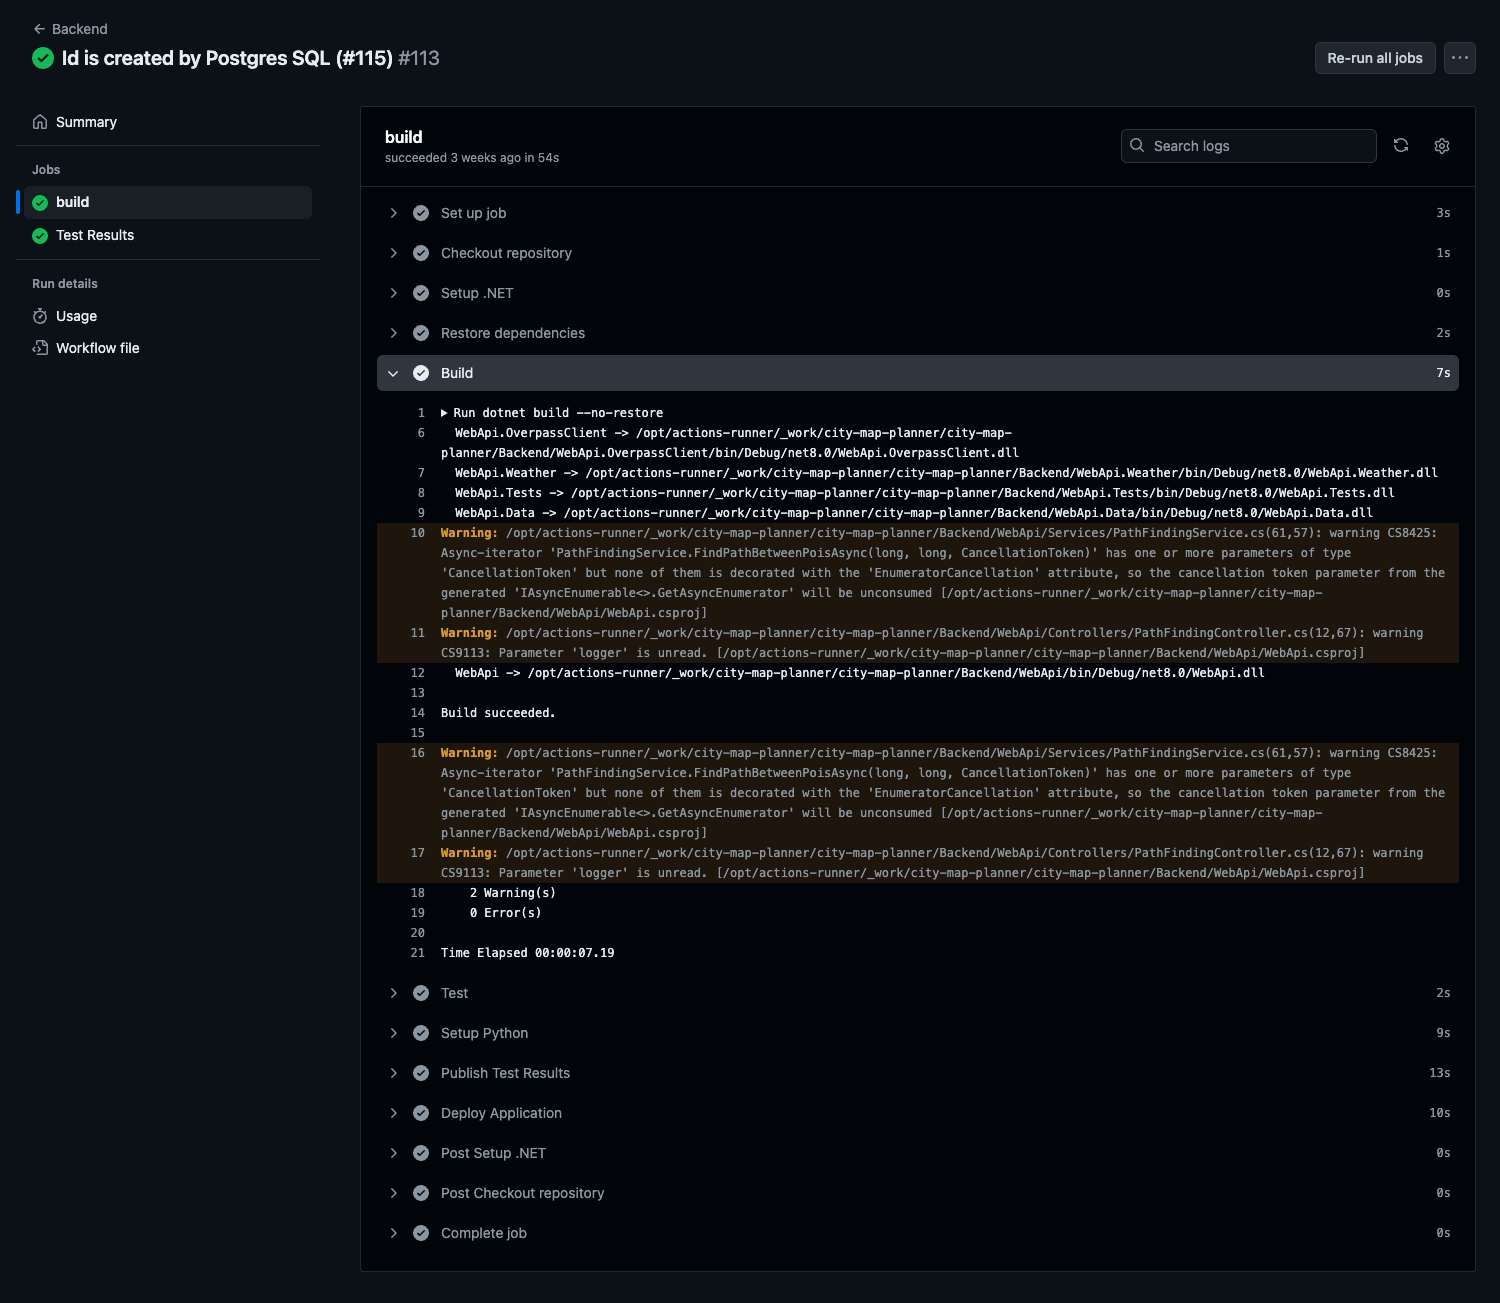
\includegraphics[width=1\textwidth]{attachments/backend-ci}
    \caption{Screenshot potoku Backendu}
\end{figure}

\subsubsection{Uprawnienia}
\begin{itemize}
    \item \texttt{\textcolor{codeblue}{contents: read}} - pozwala na odczytanie zawartości repozytorium.
    \item \texttt{\textcolor{codeblue}{issues: read}} - pozwala na odczytanie zgłoszeń.
    \item \texttt{\textcolor{codeblue}{checks: write}} - pozwala na zapis wyników kontroli.
    \item \texttt{\textcolor{codeblue}{pull-requests: write}} - pozwala na zapis pull requestów.
\end{itemize}

\subsubsection{Wydarzenia Wyzwalające Przepływ Pracy}
\begin{itemize}
    \item \texttt{\textcolor{codeblue}{workflow\_dispatch}}: ręczne uruchomienie przepływu pracy z wymaganym polem \texttt{\textcolor{codeblue}{reason}}, które musi być dostarczone przez użytkownika.
    \item \texttt{\textcolor{codeblue}{push}}: wyzwalane przy wypychaniu zmian do ścieżki \texttt{\textcolor{codeblue}{Backend/**}} na gałęzi \texttt{\textcolor{codeblue}{main}}.
    \item \texttt{\textcolor{codeblue}{pull\_request}}: wyzwalane przy tworzeniu pull requestów, które dotyczą ścieżki \texttt{\textcolor{codeblue}{Backend/**}} na gałęzi \texttt{\textcolor{codeblue}{main}}.
\end{itemize}

\subsubsection{Zadanie: build}
Uruchamiane na hoście \texttt{\textcolor{codeblue}{self-hosted}}.
\paragraph{Kroki:}
\subparagraph{Checkout repository}: Pobiera kod z repozytorium.
\begin{lstlisting}[style=yaml-colored]
    - @name@: !'Checkout repository'!
      @uses@: !'actions/checkout@v3'!
\end{lstlisting}

\subparagraph{Setup .NET}: Konfiguruje środowisko .NET w wersji 8.x.
\begin{lstlisting}[style=yaml-colored]
    - @name@: !'Setup .NET'!
      @uses@: !'actions/setup-dotnet@v3'!
      @with@:
        @dotnet-version@: !'8.x'!
\end{lstlisting}

\subparagraph{Restore dependencies}: Przywraca zależności projektu w katalogu \texttt{\textcolor{codeblue}{Backend}}.
\begin{lstlisting}[style=yaml-colored]
    - @name@: !'Restore dependencies'!
      @run@: !'dotnet restore'!
      @working-directory@: !'Backend'!
\end{lstlisting}

\subparagraph{Build}: Buduje projekt bez przywracania zależności w katalogu \texttt{\textcolor{codeblue}{Backend}}.
\begin{lstlisting}[style=yaml-colored]
    - @name@: !'Build'!
      @run@: !'dotnet build --no-restore'!
      @working-directory@: !'Backend'!
\end{lstlisting}

\subparagraph{Test}: Uruchamia testy jednostkowe z loggerem \texttt{\textcolor{codeblue}{trx}}, bez ponownego budowania projektu w katalogu \texttt{\textcolor{codeblue}{Backend}}.
\begin{lstlisting}[style=yaml-colored]
    - @name@: !'Test'!
      @run@: !'dotnet test --logger trx --no-build --verbosity normal'!
      @working-directory@: !'Backend'!
\end{lstlisting}

\subparagraph{Setup Python}: Konfiguruje środowisko Pythona w wersji 3.8, potrzebne do publikowania wyników testów.
\begin{lstlisting}[style=yaml-colored]
    - @name@: !'Setup Python'! # For publish test results
      @uses@: !'deadsnakes/action@v3.1.0'!
      @with@:
        @python-version@: !3.8!
\end{lstlisting}

\subparagraph{Publish Test Results}: Publikuje wyniki testów jednostkowych, używając plików \texttt{\textcolor{codeblue}{.trx}} z katalogu \texttt{\textcolor{codeblue}{Backend}}.
\begin{lstlisting}[style=yaml-colored]
    - @name@: !'Publish Test Results'!
      @uses@: !'EnricoMi/publish-unit-test-result-action/composite@v2'!
      @if@: !always()!
      @with@:
        @files@: |
          !Backend/**/*.trx!
\end{lstlisting}

\subparagraph{Deploy Application}: Publikuje aplikację na runtime \texttt{\textcolor{codeblue}{linux-arm64}} jako aplikację samodzielną, w trybie produkcyjnym, a następnie uruchamia skrypt \texttt{\textcolor{codeblue}{deploy.sh}} w katalogu \texttt{\textcolor{codeblue}{Backend}}. Ten krok jest pomijany, jeśli wydarzenie jest pull requestem.
\begin{lstlisting}[style=yaml-colored]
    - @name@: !'Deploy Application'!
      @run@: |
        !dotnet publish --runtime linux-arm64 --self-contained -c production WebApi!
        !./deploy.sh!
      @working-directory@: !'Backend'!
      # Do not run deployment from PR
      @if@: !github.event_name != 'pull_request'!
\end{lstlisting}

Ten przepływ pracy automatyzuje proces budowania, testowania i wdrażania projektu .NET za każdym razem, gdy zmiany są wypychane do głównej gałęzi lub gdy tworzone są pull requesty, zapewniając, że tylko zatwierdzone zmiany są wdrażane.

\subsubsection{Kod YAML}
\begin{lstlisting}[style=yaml-colored]
@name@: !'Backend'!
@permissions@:
  @contents@: !read!
  @issues@: !read!
  @checks@: !write!
  @pull-requests@: !write!

@on@:
  @workflow_dispatch@:
    @inputs@:
      @reason@:
        @description@: !'Provide reason behind manual action run'!
        @required@: !true!
        @type@: !'string'!
  @push@:
    @paths@:
    - !'Backend/**'!
    @branches@: [ !'main'! ]
  @pull_request@:
    @paths@:
    - !'Backend/**'!
    @branches@: [ !'main'! ]

@jobs@:
  @build@:
    @runs-on@: !'self-hosted'!
    @steps@:
    - @name@: !'Checkout repository'!
      @uses@: !'actions/checkout@v3'!

    - @name@: !'Setup .NET'!
      @uses@: !'actions/setup-dotnet@v3'!
      @with@:
        @dotnet-version@: !'8.x'!

    - @name@: !'Restore dependencies'!
      @run@: !'dotnet restore'!
      @working-directory@: !'Backend'!

    - @name@: !'Build'!
      @run@: !'dotnet build --no-restore'!
      @working-directory@: !'Backend'!

    - @name@: !'Test'!
      @run@: !'dotnet test --logger trx --no-build --verbosity normal'!
      @working-directory@: !'Backend'!

    - @name@: !'Setup Python'! # For publish test results
      @uses@: !'deadsnakes/action@v3.1.0'!
      @with@:
        @python-version@: !3.8!

    - @name@: !'Publish Test Results'!
      @uses@: !'EnricoMi/publish-unit-test-result-action/composite@v2'!
      @if@: !always()!
      @with@:
        @files@: |
          !Backend/**/*.trx!

    - @name@: !'Deploy Application'!
      @run@: |
        !dotnet publish --runtime linux-arm64 --self-contained -c production WebApi!
        !./deploy.sh!
      @working-directory@: !'Backend'!
      # Do not run deployment from PR
      @if@: !github.event_name != 'pull_request'!
\end{lstlisting}

\subsection{Potok Frontendu}
\label{subsec:potok-frontendu}

\begin{figure}[H]
    \centering
    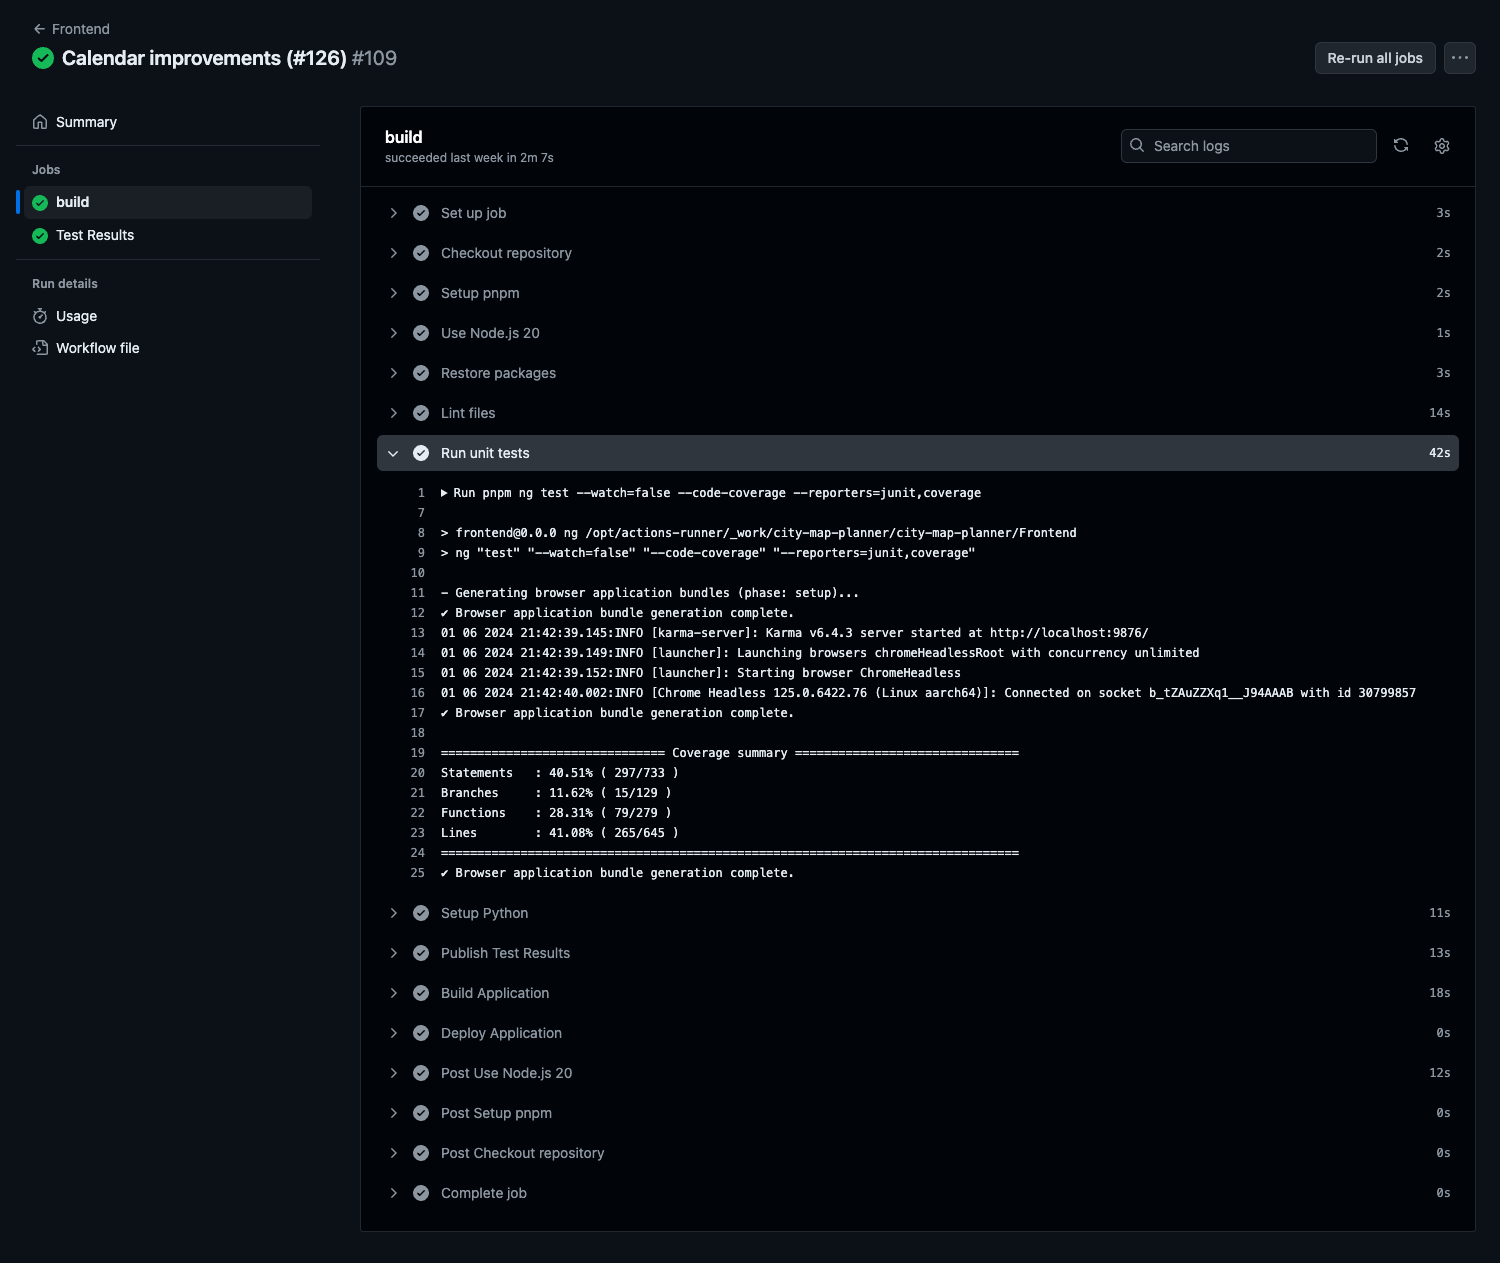
\includegraphics[width=1\textwidth]{attachments/frontend-ci}
    \caption{Screenshot potoku Frontendu}
\end{figure}

\subsubsection{Uprawnienia}
\begin{itemize}
    \item \texttt{\textcolor{codeblue}{contents: read}} - pozwala na odczytanie zawartości repozytorium.
    \item \texttt{\textcolor{codeblue}{issues: read}} - pozwala na odczytanie zgłoszeń.
    \item \texttt{\textcolor{codeblue}{checks: write}} - pozwala na zapis wyników kontroli.
    \item \texttt{\textcolor{codeblue}{pull-requests: write}} - pozwala na zapis pull requestów.
\end{itemize}

\subsubsection{Wydarzenia Wyzwalające Przepływ Pracy}
\begin{itemize}
    \item \texttt{\textcolor{codeblue}{workflow\_dispatch}}: ręczne uruchomienie przepływu pracy z wymaganym polem \texttt{\textcolor{codeblue}{reason}}, które musi być dostarczone przez użytkownika.
    \item \texttt{\textcolor{codeblue}{push}}: wyzwalane przy wypychaniu zmian do ścieżki \texttt{\textcolor{codeblue}{Frontend/**}} na gałęzi \texttt{\textcolor{codeblue}{main}}.
    \item \texttt{\textcolor{codeblue}{pull\_request}}: wyzwalane przy tworzeniu pull requestów, które dotyczą ścieżki \texttt{\textcolor{codeblue}{Frontend/**}} na gałęzi \texttt{\textcolor{codeblue}{main}}.
\end{itemize}

\subsubsection{Zadania}
Uruchamiane na hoście \texttt{\textcolor{codeblue}{self-hosted}}.
\paragraph{Kroki:}
\subparagraph{Checkout repository}: Pobiera kod z repozytorium.
\begin{lstlisting}[style=yaml-colored]
    - +name+: !'Checkout repository'!
      +uses+: !'actions/checkout@v3'!
\end{lstlisting}

\subparagraph{Setup pnpm}: Konfiguruje pnpm w wersji 9.
\begin{lstlisting}[style=yaml-colored]
    - +name+: !'Setup pnpm'!
      +uses+: !'pnpm/action-setup@v2'!
      +with+:
        +version+: !9!
\end{lstlisting}

\subparagraph{Use Node.js 20}: Ustawia Node.js w wersji 20.x, z buforowaniem pnpm.
\begin{lstlisting}[style=yaml-colored]
    - +name+: !'Use Node.js 20'!
      +uses+: !'actions/setup-node@v3'!
      +with+:
        +node-version+: !'20.x'!
        +cache+: !'pnpm'!
        +cache-dependency-path+: !'Frontend/pnpm-lock.yaml'!
\end{lstlisting}

\subparagraph{Restore packages}: Przywraca pakiety pnpm.
\begin{lstlisting}[style=yaml-colored]
    - +name+: !'Restore packages'!
      +run+: |
        !corepack enable!
        !pnpm config set store-dir $RUNNER_TOOL_CACHE/.pnpm!
        !pnpm i --frozen-lockfile!
      +working-directory+: !'Frontend'!
\end{lstlisting}

\subparagraph{Lint files}: Sprawdza pliki za pomocą pnpm lint.
\begin{lstlisting}[style=yaml-colored]
    - +name+: !'Lint files'!
      +run+: !'pnpm ng lint'!
      +working-directory+: !'Frontend'!
\end{lstlisting}

\subparagraph{Run unit tests}: Uruchamia testy jednostkowe z generowaniem raportu pokrycia kodu.
\begin{lstlisting}[style=yaml-colored]
    - +name+: !'Run unit tests'!
      +run+: !'pnpm ng test --watch=false --code-coverage --reporters=junit,coverage'!
      +working-directory+: !'Frontend'!
      +env+:
        +CHROME_BIN+: !'/usr/bin/chromium-browser'!
\end{lstlisting}

\subparagraph{Setup Python}: Konfiguruje środowisko Pythona w wersji 3.8, potrzebne do publikowania wyników testów.
\begin{lstlisting}[style=yaml-colored]
    - +name+: !'Setup Python'! # For publish test results
      +uses+: !'deadsnakes/action@v3.1.0'!
      +with+:
        +python-version+: !3.8!
\end{lstlisting}

\subparagraph{Publish Test Results}: Publikuje wyniki testów jednostkowych, używając plików \texttt{\textcolor{codeblue}{.xml}} z katalogu \texttt{\textcolor{codeblue}{Frontend}}.
\begin{lstlisting}[style=yaml-colored]
    - +name+: !'Publish Test Results'!
      +uses+: !'EnricoMi/publish-unit-test-result-action/composite@v2'!
      +if+: !always()!
      +with+:
        +files+: |
          !Frontend/coverage/**/TESTS*.xml!
\end{lstlisting}

\subparagraph{Build Application}: Buduje aplikację.
\begin{lstlisting}[style=yaml-colored]
    - +name+: !'Build Application'!
      +run+: !'pnpm build'!
      +working-directory+: !'Frontend'!
\end{lstlisting}

\subparagraph{Deploy Application}: Wdraża aplikację, uruchamiając skrypt \texttt{\textcolor{codeblue}{deploy.sh}} w katalogu \texttt{\textcolor{codeblue}{Frontend}}. Ten krok jest pomijany, jeśli wydarzenie jest pull requestem.
\begin{lstlisting}[style=yaml-colored]
    - +name+: !'Deploy Application'!
      +run+: !'./deploy.sh'!
      +working-directory+: !'Frontend'!
      # Do not run deployment from PR
      +if+: !github.event_name != 'pull_request'!
\end{lstlisting}

Ten przepływ pracy automatyzuje proces instalacji zależności, buforowania, budowania kodu i uruchamiania testów jednostkowych za każdym razem, gdy zmiany są wypychane do głównej gałęzi lub gdy tworzone są pull requesty, zapewniając, że tylko zatwierdzone zmiany są wdrażane.

\subsubsection{Kod YAML}
\begin{lstlisting}[style=yaml-colored]
+name+: !'Frontend'!
+permissions+:
  +contents+: !read!
  +issues+: !read!
  +checks+: !write!
  +pull-requests+: !write!

+on+:
  +workflow_dispatch+:
    +inputs+:
      +reason+:
        +description+: !'Provide reason behind manual action run'!
        +required+: !true!
        +type+: !'string'!
  +push+:
    +paths+:
    - !'Frontend/**'!
    +branches+: [ !'main'! ]
  +pull_request+:
    +paths+:
    - !'Frontend/**'!
    +branches+: [ !'main'! ]

+jobs+:
  +build+:
    +runs-on+: !'self-hosted'!
    +steps+:
    - +name+: !'Checkout repository'!
      +uses+: !'actions/checkout@v3'!

    - +name+: !'Setup pnpm'!
      +uses+: !'pnpm/action-setup@v2'!
      +with+:
        +version+: !9!

    - +name+: !'Use Node.js 20'!
      +uses+: !'actions/setup-node@v3'!
      +with+:
        +node-version+: !'20.x'!
        +cache+: !'pnpm'!
        +cache-dependency-path+: !'Frontend/pnpm-lock.yaml'!

    - +name+: !'Restore packages'!
      +run+: |
        !corepack enable!
        !pnpm config set store-dir $RUNNER_TOOL_CACHE/.pnpm!
        !pnpm i --frozen-lockfile!
      +working-directory+: !'Frontend'!

    - +name+: !'Lint files'!
      +run+: !'pnpm ng lint'!
      +working-directory+: !'Frontend'!

    - +name+: !'Run unit tests'!
      +run+: !'pnpm ng test --watch=false --code-coverage --reporters=junit,coverage'!
      +working-directory+: !'Frontend'!
      +env+:
        +CHROME_BIN+: !'/usr/bin/chromium-browser'!

    - +name+: !'Setup Python'! # For publish test results
      +uses+: !'deadsnakes/action@v3.1.0'!
      +with+:
        +python-version+: !3.8!

    - +name+: !'Publish Test Results'!
      +uses+: !'EnricoMi/publish-unit-test-result-action/composite@v2'!
      +if+: !always()!
      +with+:
        +files+: |
          !Frontend/coverage/**/TESTS*.xml!

    - +name+: !'Build Application'!
      +run+: !'pnpm build'!
      +working-directory+: !'Frontend'!

    - +name+: !'Deploy Application'!
      +run+: !'./deploy.sh'!
      +working-directory+: !'Frontend'!
      # Do not run deployment from PR
      +if+: !github.event_name != 'pull_request'!
\end{lstlisting}

\subsection{Potok Dokumentacji}
\label{subsec:potok-dokumentacji}

\begin{figure}[H]
    \centering
    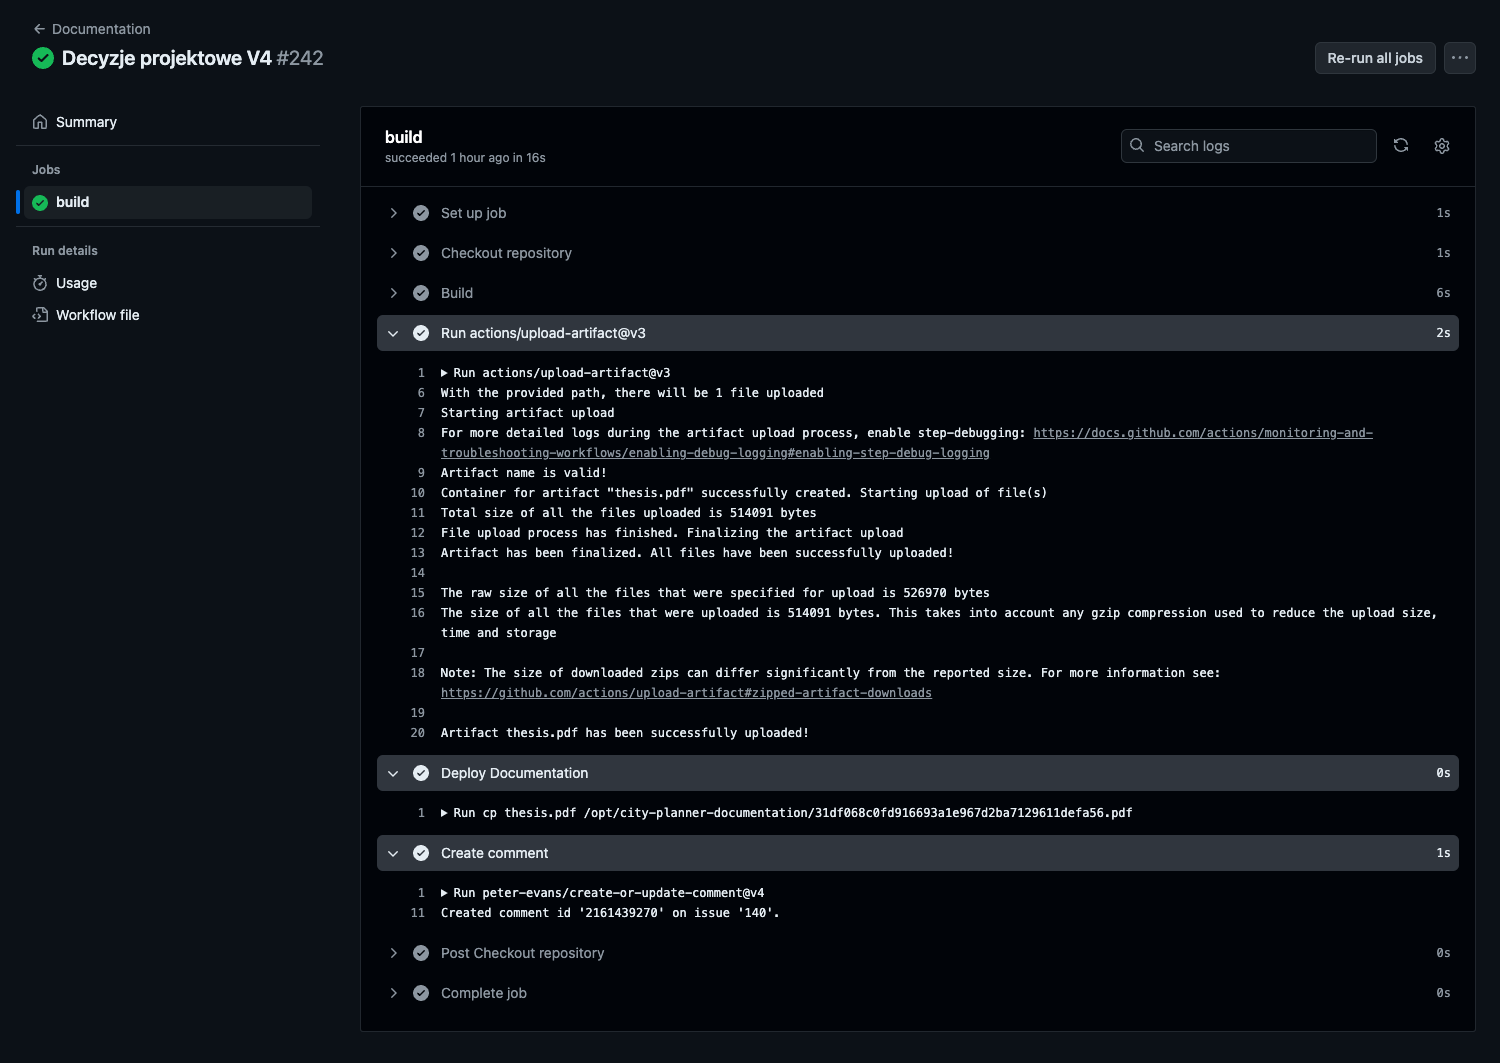
\includegraphics[width=1\textwidth]{attachments/docs-ci}
    \caption{Screenshot potoku dokumentacji}
\end{figure}

\begin{figure}[H]
    \centering
    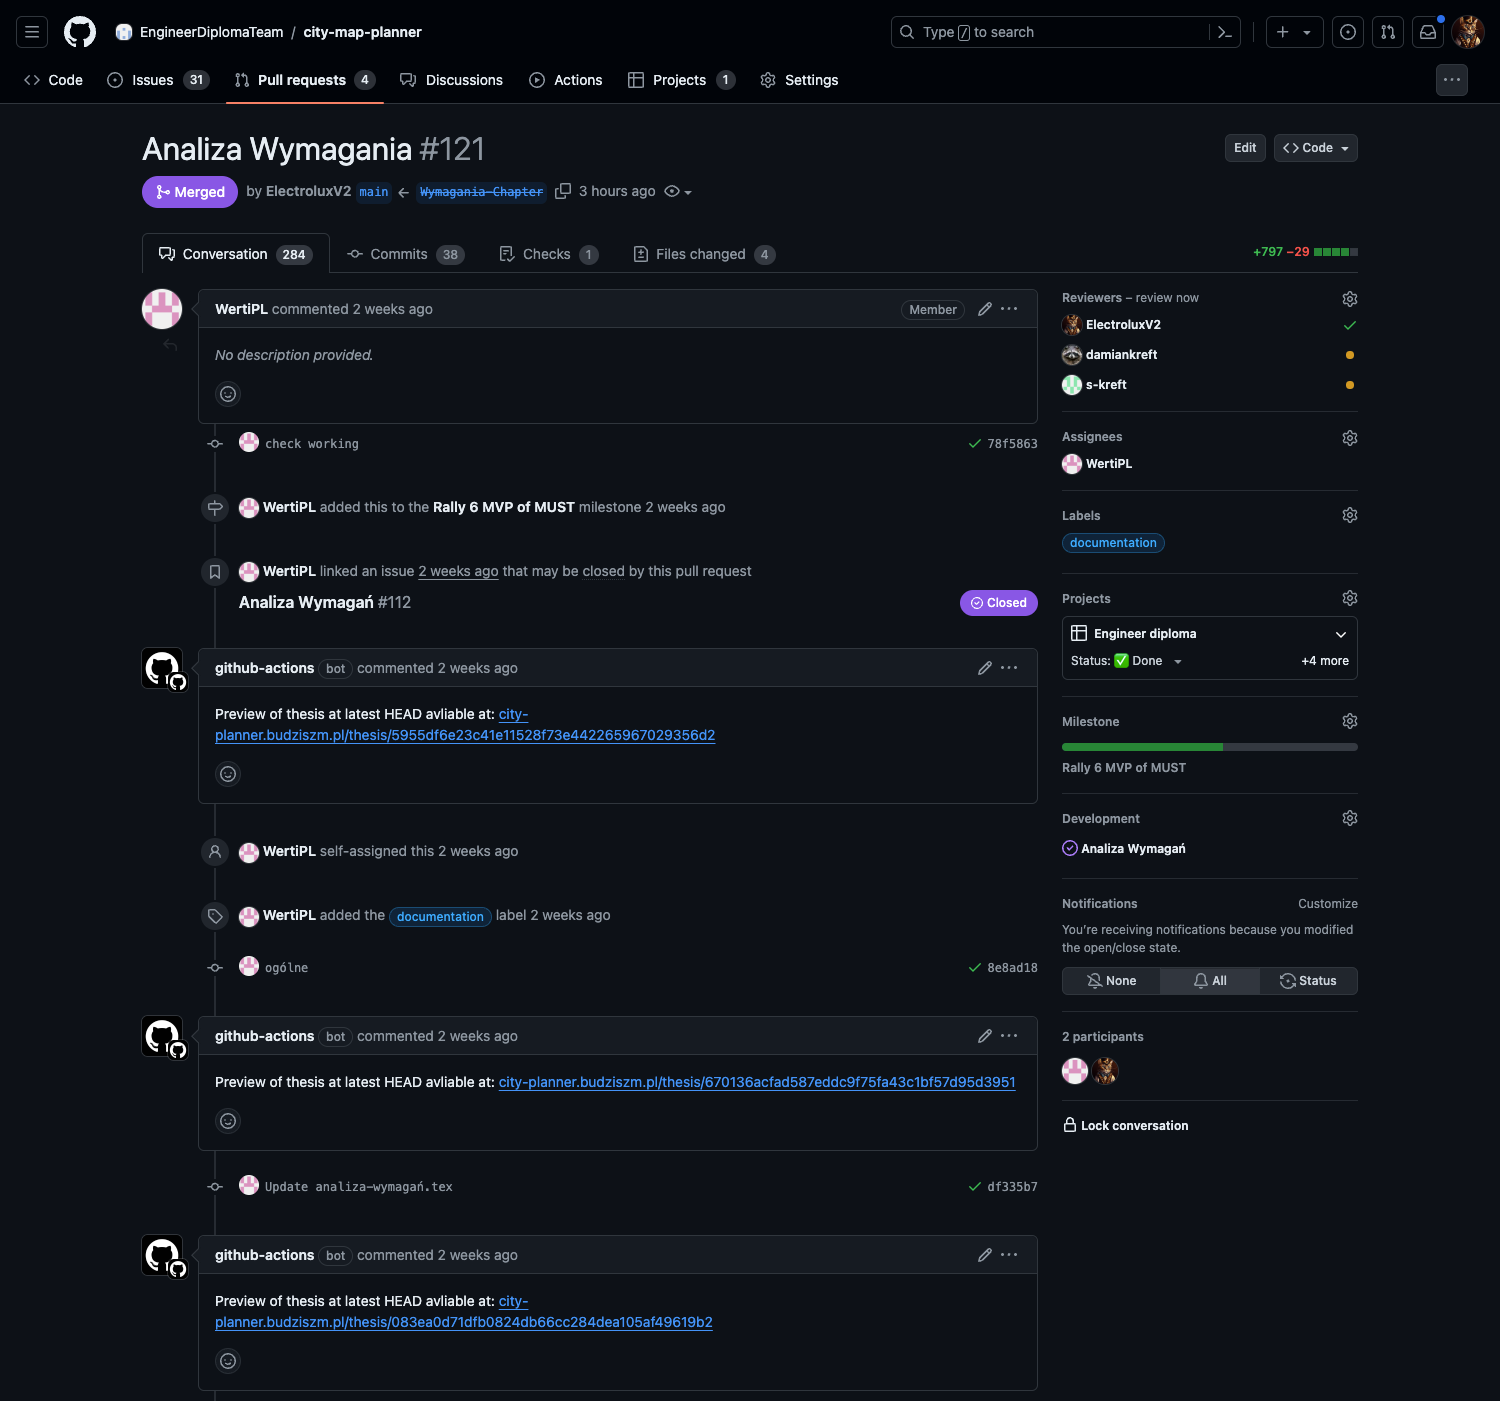
\includegraphics[width=1\textwidth]{attachments/docs-pr}
    \caption{Screenshot komentarza w widoku Pull Request}
\end{figure}

\subsubsection{Uprawnienia}
\begin{itemize}
    \item \texttt{\textcolor{codeblue}{contents: read}} - pozwala na odczytanie zawartości repozytorium.
    \item \texttt{\textcolor{codeblue}{issues: read}} - pozwala na odczytanie zgłoszeń.
    \item \texttt{\textcolor{codeblue}{checks: write}} - pozwala na zapis wyników kontroli.
    \item \texttt{\textcolor{codeblue}{pull-requests: write}} - pozwala na zapis pull requestów.
\end{itemize}

\subsubsection{Wydarzenia Wyzwalające Przepływ Pracy}
\begin{itemize}
    \item \texttt{\textcolor{codeblue}{workflow\_dispatch}}: ręczne uruchomienie przepływu pracy z wymaganym polem \texttt{\textcolor{codeblue}{reason}}, które musi być dostarczone przez użytkownika.
    \item \texttt{\textcolor{codeblue}{push}}: wyzwalane przy wypychaniu zmian do ścieżki \texttt{\textcolor{codeblue}{Documentation/**}} na gałęzi \texttt{\textcolor{codeblue}{main}}.
    \item \texttt{\textcolor{codeblue}{pull\_request}}: wyzwalane przy tworzeniu pull requestów, które dotyczą ścieżki \texttt{\textcolor{codeblue}{Documentation/**}} na gałęzi \texttt{\textcolor{codeblue}{main}}.
\end{itemize}

\subsubsection{Zadania}
Uruchamiane na hoście \texttt{\textcolor{codeblue}{self-hosted}}.
\paragraph{Kroki:}
\subparagraph{Checkout repository}: Pobiera kod z repozytorium.
\begin{lstlisting}[style=yaml-colored]
    - +name+: !'Checkout repository'!
      +uses+: !'actions/checkout@v3'!
\end{lstlisting}

\subparagraph{Build}: Buduje dokumentację LaTeX, uruchamiając komendy `pdflatex`, `biber`, `makeglossaries` i ponownie `pdflatex` w katalogu \texttt{\textcolor{codeblue}{Documentation}}.
\begin{lstlisting}[style=yaml-colored]
    - +name+: !'Build'!
      # Glossaries https://tex.stackexchange.com/a/46732
      # Run build twice https://texfaq.org/FAQ-rerun
      +run+: |
        !pdflatex thesis.tex!
        !biber thesis!
        !makeglossaries thesis!
        !pdflatex thesis.tex!
        !pdflatex thesis.tex!
      +working-directory+: !'Documentation'!
\end{lstlisting}

\subparagraph{Upload Artifact}: Przesyła wygenerowany plik PDF jako artefakt.
\begin{lstlisting}[style=yaml-colored]
    - +uses+: !actions/upload-artifact@v3!
      +with+:
        +name+: !'thesis.pdf'!
        +path+: !'Documentation/thesis.pdf'!
\end{lstlisting}

\subparagraph{Deploy Documentation}: Kopiuje wygenerowany plik PDF do odpowiedniego katalogu w zależności od tego, czy wydarzenie jest pull requestem.
\begin{lstlisting}[style=yaml-colored]
    - +name+: !'Deploy Documentation'!
      +run+: |
        !cp thesis.pdf /opt/city-planner-documentation/${{ github.event_name == 'pull_request' && format('{0}.pdf', github.sha) || 'thesis.pdf' }}!
      +working-directory+: !'Documentation'!
\end{lstlisting}

\subparagraph{Create comment}: Tworzy komentarz w pull request, zawierający link do wygenerowanej dokumentacji.
\begin{lstlisting}[style=yaml-colored]
    - +name+: !'Create comment'!
      +uses+: !peter-evans/create-or-update-comment@v4!
      +with+:
        +issue-number+: ${{ github.event.number }}
        +body+: |
            !Preview of thesis at latest HEAD available at: [https://city-planner.budziszm.pl/thesis/${{ github.sha }}](https://city-planner.budziszm.pl/thesis/${{ github.sha }})!
      # Comment only on PR
      +if+: !github.event_name == 'pull_request'!
\end{lstlisting}

Ten przepływ pracy automatyzuje proces budowania i wdrażania dokumentacji LaTeX za każdym razem, gdy zmiany są wypychane do głównej gałęzi lub gdy tworzone są pull requesty, zapewniając, że tylko zatwierdzone zmiany są wdrażane.

\subsubsection{Kod YAML}
\begin{lstlisting}[style=yaml-colored]
+name+: !'Documentation'!
+permissions+:
  +contents+: !read!
  +issues+: !read!
  +checks+: !write!
  +pull-requests+: !write!

+on+:
  +workflow_dispatch+:
    +inputs+:
      +reason+:
        +description+: !'Provide reason behind manual action run'!
        +required+: !true!
        +type+: !'string'!
  +push+:
    +paths+:
    - !'Documentation/**'!
    +branches+: [ !'main'! ]
  +pull_request+:
    +paths+:
    - !'Documentation/**'!
    +branches+: [ !'main'! ]

+jobs+:
  +build+:
    +runs-on+: !'self-hosted'!
    +steps+:
    - +name+: !'Checkout repository'!
      +uses+: !'actions/checkout@v3'!

    - +name+: !'Build'!
      # Glossaries https://tex.stackexchange.com/a/46732
      # Run build twice https://texfaq.org/FAQ-rerun
      +run+: |
        !pdflatex thesis.tex!
        !biber thesis!
        !makeglossaries thesis!
        !pdflatex thesis.tex!
        !pdflatex thesis.tex!
      +working-directory+: !'Documentation'!

    - +uses+: !actions/upload-artifact@v3!
      +with+:
        +name+: !'thesis.pdf'!
        +path+: !'Documentation/thesis.pdf'!

    - +name+: !'Deploy Documentation'!
      +run+: |
        !cp thesis.pdf /opt/city-planner-documentation/${{ github.event_name == 'pull_request' && format('{0}.pdf', github.sha) || 'thesis.pdf' }}!
      +working-directory+: !'Documentation'!

    - +name+: !'Create comment'!
      +uses+: !peter-evans/create-or-update-comment@v4!
      +with+:
        +issue-number+: !${{ github.event.number }}!
        +body+: |
            !Preview of thesis at latest HEAD available at: [https://city-planner.budziszm.pl/thesis/${{ github.sha }}](https://city-planner.budziszm.pl/thesis/${{ github.sha }})!
      # Comment only on PR
      +if+: !github.event_name == 'pull_request'!
\end{lstlisting}
